% Options for packages loaded elsewhere
\PassOptionsToPackage{unicode}{hyperref}
\PassOptionsToPackage{hyphens}{url}
%
\documentclass[
]{book}
\usepackage{amsmath,amssymb}
\usepackage{lmodern}
\usepackage{iftex}
\ifPDFTeX
  \usepackage[T1]{fontenc}
  \usepackage[utf8]{inputenc}
  \usepackage{textcomp} % provide euro and other symbols
\else % if luatex or xetex
  \usepackage{unicode-math}
  \defaultfontfeatures{Scale=MatchLowercase}
  \defaultfontfeatures[\rmfamily]{Ligatures=TeX,Scale=1}
\fi
% Use upquote if available, for straight quotes in verbatim environments
\IfFileExists{upquote.sty}{\usepackage{upquote}}{}
\IfFileExists{microtype.sty}{% use microtype if available
  \usepackage[]{microtype}
  \UseMicrotypeSet[protrusion]{basicmath} % disable protrusion for tt fonts
}{}
\makeatletter
\@ifundefined{KOMAClassName}{% if non-KOMA class
  \IfFileExists{parskip.sty}{%
    \usepackage{parskip}
  }{% else
    \setlength{\parindent}{0pt}
    \setlength{\parskip}{6pt plus 2pt minus 1pt}}
}{% if KOMA class
  \KOMAoptions{parskip=half}}
\makeatother
\usepackage{xcolor}
\usepackage{color}
\usepackage{fancyvrb}
\newcommand{\VerbBar}{|}
\newcommand{\VERB}{\Verb[commandchars=\\\{\}]}
\DefineVerbatimEnvironment{Highlighting}{Verbatim}{commandchars=\\\{\}}
% Add ',fontsize=\small' for more characters per line
\usepackage{framed}
\definecolor{shadecolor}{RGB}{248,248,248}
\newenvironment{Shaded}{\begin{snugshade}}{\end{snugshade}}
\newcommand{\AlertTok}[1]{\textcolor[rgb]{0.94,0.16,0.16}{#1}}
\newcommand{\AnnotationTok}[1]{\textcolor[rgb]{0.56,0.35,0.01}{\textbf{\textit{#1}}}}
\newcommand{\AttributeTok}[1]{\textcolor[rgb]{0.77,0.63,0.00}{#1}}
\newcommand{\BaseNTok}[1]{\textcolor[rgb]{0.00,0.00,0.81}{#1}}
\newcommand{\BuiltInTok}[1]{#1}
\newcommand{\CharTok}[1]{\textcolor[rgb]{0.31,0.60,0.02}{#1}}
\newcommand{\CommentTok}[1]{\textcolor[rgb]{0.56,0.35,0.01}{\textit{#1}}}
\newcommand{\CommentVarTok}[1]{\textcolor[rgb]{0.56,0.35,0.01}{\textbf{\textit{#1}}}}
\newcommand{\ConstantTok}[1]{\textcolor[rgb]{0.00,0.00,0.00}{#1}}
\newcommand{\ControlFlowTok}[1]{\textcolor[rgb]{0.13,0.29,0.53}{\textbf{#1}}}
\newcommand{\DataTypeTok}[1]{\textcolor[rgb]{0.13,0.29,0.53}{#1}}
\newcommand{\DecValTok}[1]{\textcolor[rgb]{0.00,0.00,0.81}{#1}}
\newcommand{\DocumentationTok}[1]{\textcolor[rgb]{0.56,0.35,0.01}{\textbf{\textit{#1}}}}
\newcommand{\ErrorTok}[1]{\textcolor[rgb]{0.64,0.00,0.00}{\textbf{#1}}}
\newcommand{\ExtensionTok}[1]{#1}
\newcommand{\FloatTok}[1]{\textcolor[rgb]{0.00,0.00,0.81}{#1}}
\newcommand{\FunctionTok}[1]{\textcolor[rgb]{0.00,0.00,0.00}{#1}}
\newcommand{\ImportTok}[1]{#1}
\newcommand{\InformationTok}[1]{\textcolor[rgb]{0.56,0.35,0.01}{\textbf{\textit{#1}}}}
\newcommand{\KeywordTok}[1]{\textcolor[rgb]{0.13,0.29,0.53}{\textbf{#1}}}
\newcommand{\NormalTok}[1]{#1}
\newcommand{\OperatorTok}[1]{\textcolor[rgb]{0.81,0.36,0.00}{\textbf{#1}}}
\newcommand{\OtherTok}[1]{\textcolor[rgb]{0.56,0.35,0.01}{#1}}
\newcommand{\PreprocessorTok}[1]{\textcolor[rgb]{0.56,0.35,0.01}{\textit{#1}}}
\newcommand{\RegionMarkerTok}[1]{#1}
\newcommand{\SpecialCharTok}[1]{\textcolor[rgb]{0.00,0.00,0.00}{#1}}
\newcommand{\SpecialStringTok}[1]{\textcolor[rgb]{0.31,0.60,0.02}{#1}}
\newcommand{\StringTok}[1]{\textcolor[rgb]{0.31,0.60,0.02}{#1}}
\newcommand{\VariableTok}[1]{\textcolor[rgb]{0.00,0.00,0.00}{#1}}
\newcommand{\VerbatimStringTok}[1]{\textcolor[rgb]{0.31,0.60,0.02}{#1}}
\newcommand{\WarningTok}[1]{\textcolor[rgb]{0.56,0.35,0.01}{\textbf{\textit{#1}}}}
\usepackage{longtable,booktabs,array}
\usepackage{calc} % for calculating minipage widths
% Correct order of tables after \paragraph or \subparagraph
\usepackage{etoolbox}
\makeatletter
\patchcmd\longtable{\par}{\if@noskipsec\mbox{}\fi\par}{}{}
\makeatother
% Allow footnotes in longtable head/foot
\IfFileExists{footnotehyper.sty}{\usepackage{footnotehyper}}{\usepackage{footnote}}
\makesavenoteenv{longtable}
\usepackage{graphicx}
\makeatletter
\def\maxwidth{\ifdim\Gin@nat@width>\linewidth\linewidth\else\Gin@nat@width\fi}
\def\maxheight{\ifdim\Gin@nat@height>\textheight\textheight\else\Gin@nat@height\fi}
\makeatother
% Scale images if necessary, so that they will not overflow the page
% margins by default, and it is still possible to overwrite the defaults
% using explicit options in \includegraphics[width, height, ...]{}
\setkeys{Gin}{width=\maxwidth,height=\maxheight,keepaspectratio}
% Set default figure placement to htbp
\makeatletter
\def\fps@figure{htbp}
\makeatother
\setlength{\emergencystretch}{3em} % prevent overfull lines
\providecommand{\tightlist}{%
  \setlength{\itemsep}{0pt}\setlength{\parskip}{0pt}}
\setcounter{secnumdepth}{5}
\usepackage{booktabs}
\ifLuaTeX
  \usepackage{selnolig}  % disable illegal ligatures
\fi
\usepackage[]{natbib}
\bibliographystyle{plainnat}
\IfFileExists{bookmark.sty}{\usepackage{bookmark}}{\usepackage{hyperref}}
\IfFileExists{xurl.sty}{\usepackage{xurl}}{} % add URL line breaks if available
\urlstyle{same} % disable monospaced font for URLs
\hypersetup{
  pdftitle={SDMX Constructor: User Manual},
  pdfauthor={International Labour Organization: Department of Statistics},
  hidelinks,
  pdfcreator={LaTeX via pandoc}}

\title{SDMX Constructor: User Manual}
\author{International Labour Organization: Department of Statistics}
\date{2023-04-24}

\usepackage{amsthm}
\newtheorem{theorem}{Theorem}[chapter]
\newtheorem{lemma}{Lemma}[chapter]
\newtheorem{corollary}{Corollary}[chapter]
\newtheorem{proposition}{Proposition}[chapter]
\newtheorem{conjecture}{Conjecture}[chapter]
\theoremstyle{definition}
\newtheorem{definition}{Definition}[chapter]
\theoremstyle{definition}
\newtheorem{example}{Example}[chapter]
\theoremstyle{definition}
\newtheorem{exercise}{Exercise}[chapter]
\theoremstyle{definition}
\newtheorem{hypothesis}{Hypothesis}[chapter]
\theoremstyle{remark}
\newtheorem*{remark}{Remark}
\newtheorem*{solution}{Solution}
\begin{document}
\maketitle

{
\setcounter{tocdepth}{1}
\tableofcontents
}
\hypertarget{preface}{%
\chapter*{Preface}\label{preface}}
\addcontentsline{toc}{chapter}{Preface}

Welcome to the SDMX Constructor User Manual!

SDMX Constructor\footnote{It was previously called DSD Constructor, it supported creating and editing Data Structure Definitions (DSDs) and their related artefacts (i.e., concept schemes and code lists). The significant improvements and additions to the software justify the name change of the tool from DSD Constructor to SDMX Constructor. With the latest update, the tool can now translate SDMX artefacts in multiple languages, integrate with the .Stat Suite, and manage reference metadata. Additionally, the tool now includes Table Modeller functionalities that make it easier for users who are new to SDMX to understand and use the software. The updated software is no longer just a DSD Constructor but a complete SDMX Constructor capable of handling various aspects of SDMX data and metadata. The new name better reflects the software's expanded capabilities, making it more relevant and recognizable to the target audience (\url{https://ilostat.github.io/dsdc/}).} is a powerful desktop software tool that helps users model aggregate data per the SDMX standards \footnote{An ISO standard (since 2005, version 2.1 since 2013): \url{https://www.iso.org/obp/ui/fr/\#iso:std:iso:17369:ed-1:v1:en} and \url{https://sdmx.org/?page_id=5008}} . It eases generating and editing SDMX artefacts and ultimately supports data availability and access through SDMX-compliant data portals (such as ones built with .Stat Suite\footnote{To learn more about the .Stat Suite platform please refer to the documentation here: \url{https://siscc.org/stat-suite/}. The SDMX Constructor has been optimised to seamlessly integrate with the .Stat Suite platform, as its back-end client.} ).

SDMX Constructor is one of the tools that comprise the ILO SDMX toolkit \footnote{\url{https://ilostat.ilo.org/resources/sdmx-tools/}}, alongside SMART (Statistical Metadata-driven Analysis and Reporting Tool) and the SDMX Excel Add-in.

This user manual for the SDMX Constructor provides step-by-step instructions on using the tool in a user-friendly and accessible manner. It provides an in-depth understanding of SDMX Constructor's features and functionalities. It is an essential resource for anyone using the tool to manage and share data following the SDMX standards.

Below is a screenshot of the tool's landing page as an example of the user interface.

\begin{figure}

{\centering 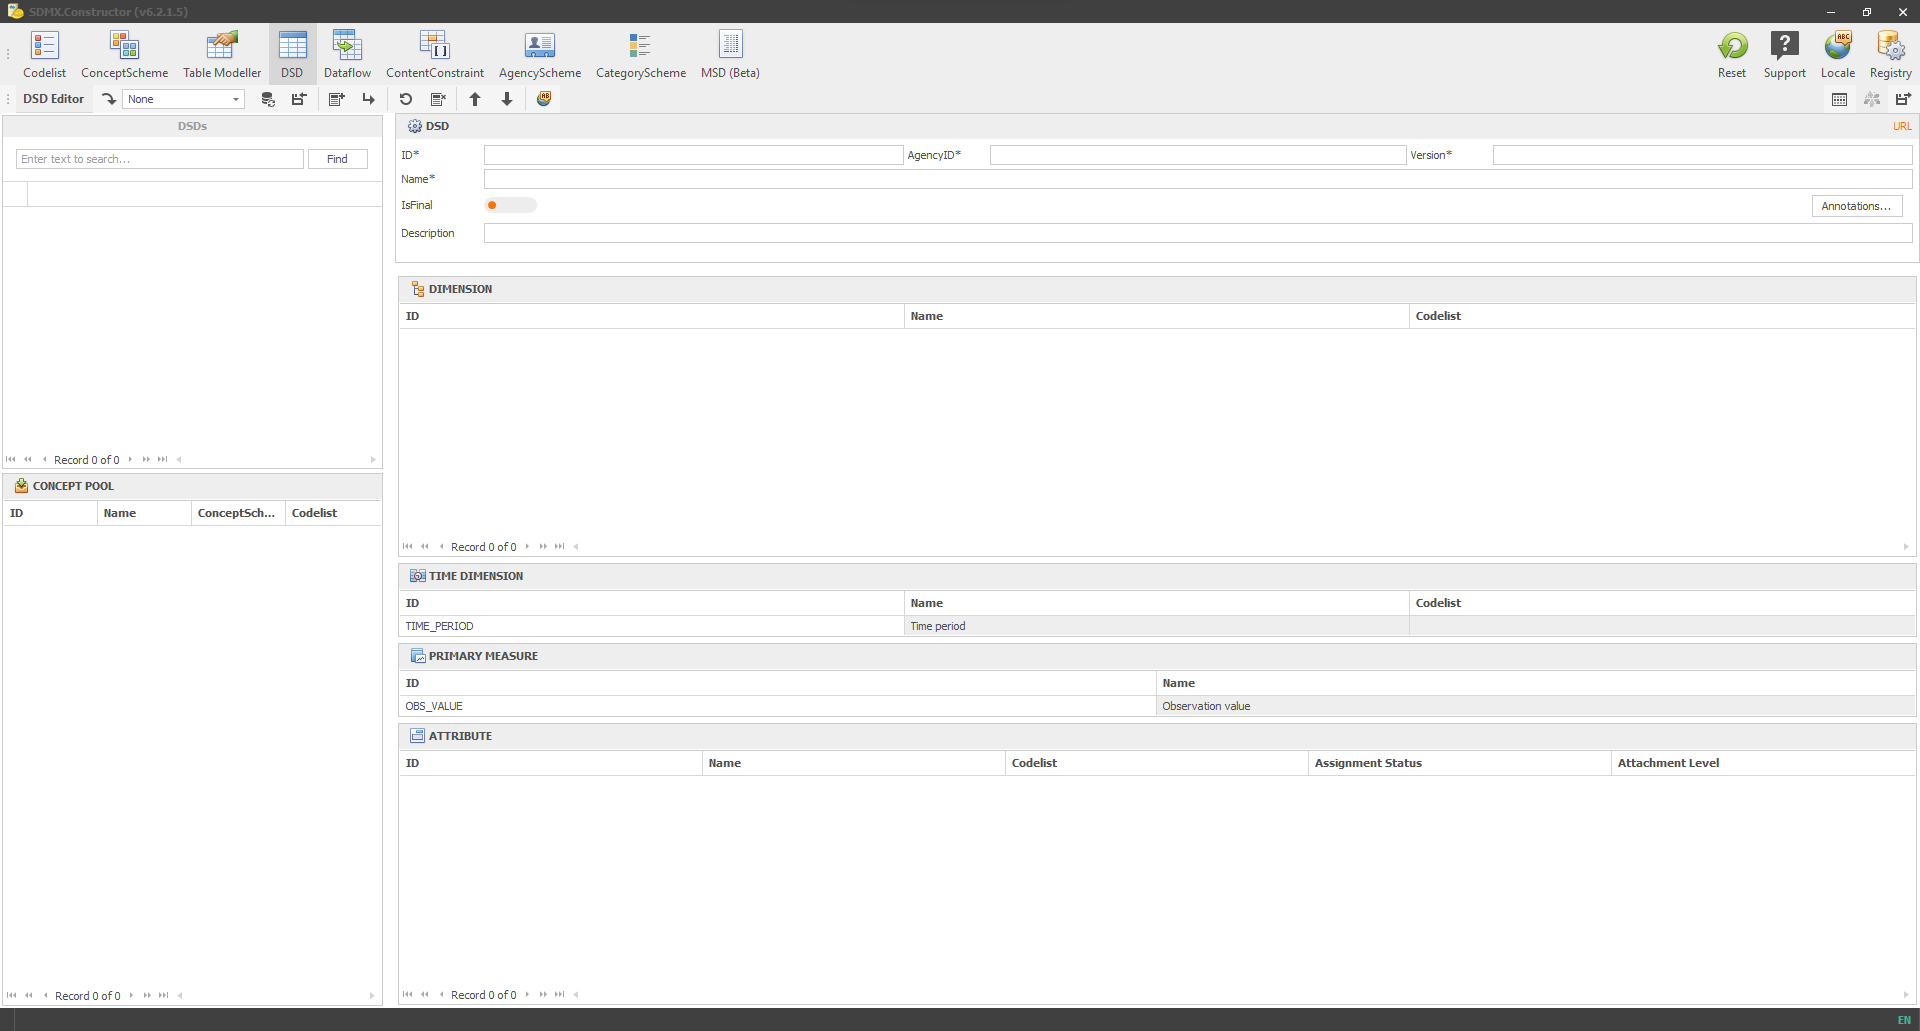
\includegraphics[width=1\linewidth]{./images/image001} 

}

\caption{A screenshot of SDMX Constructor}\label{fig:front-cover}
\end{figure}

\href{images/image001.png}{Click here to enlarge the image}

\hypertarget{audience-and-use-cases}{%
\section*{Audience and use cases}\label{audience-and-use-cases}}
\addcontentsline{toc}{section}{Audience and use cases}

The SDMX Constructor is designed to meet the needs of a wide range of users, from beginners who are new to SDMX to data managers who need advanced capabilities for managing large and complex datasets. In addition to these user types, there may be other groups of users with specific requirements or use cases. This user manual provides guidance and instructions for using the SDMX Constructor, focusing on the needs of these various user types.

\textbf{SDMX beginners}: These users are new to SDMX and want to use the SDMX Constructor to view, edit, and create new SDMX structural artefacts. They may need assistance understanding the SDMX concepts, terminology, and the software's user interface.

For SDMX beginners, this manual explains using the SDMX Constructor to access, view, edit, and create SDMX structural artefacts from SDMX registries. While one can find information on SDMX concepts and terminology from other sources, this manual focuses explicitly on the user interfaces of the SDMX Constructor. The SDMX beginners may be keen to know how to \protect\hyperlink{accessing-sdmx}{access SDMX artefacts from default SDMX registries} and \protect\hyperlink{connect-to}{connect to a new SDMX registry} from the SDMX Constructor.

\textbf{Data managers}: These users are likely familiar with the SDMX concepts and terminology and may require information about advanced functionalities offered by the SDMX Constructor. For example, they may want to use the SDMX Constructor as a backend client to manage SDMX artefacts for the .Stat Data Lifecycle Manager (DLM). For such cases, they may also use the SDMX Constructor to build the initial structural metadata when creating a new .Stat Suite instance.

There are several topics that data managers may be interested in learning when it comes to \protect\hyperlink{creating-sdmx}{creating SDMX artefacts from scratch}. Firstly, they may want to start by \protect\hyperlink{setting-up}{setting up a registry as a local folder}. Next, they can \protect\hyperlink{preparing-inputs}{prepare inputs} and create several artefacts, including the \protect\hyperlink{creating-agencyschme}{AgencyScheme}, \protect\hyperlink{creating-conceptscheme}{ConceptScheme, and Codelist} and the \protect\hyperlink{creating-dsd}{DSD, Dataflow, ContentConstraint, and CategoryScheme}. After creating these artefacts, they may want to learn how to \protect\hyperlink{upload-the}{upload the XML file to the Data Lifecycle Manager (DLM)}. Additionally, they may want to know how to \protect\hyperlink{access-sdmx}{access SDMX artefacts from default SDMX registries} and \protect\hyperlink{connect-to}{connect to a new SDMX registry} for editing SDMX artefacts directly in the DLM.

\textbf{SDMX metadata managers}: These users manage SDMX artefacts and ensure their accuracy and consistency. They may use the SDMX Constructor to model data and modify SDMX structural artefacts, including translating SDMX artefacts in various languages, managing annotations and creating Metadata Structure Definition (MSD).

\hypertarget{scope-and-assumptions}{%
\section*{Scope and assumptions}\label{scope-and-assumptions}}
\addcontentsline{toc}{section}{Scope and assumptions}

This comprehensive manual provides a step-by-step guide on getting started with the software, including installing it and creating and managing SDMX artefacts. The manual includes a detailed overview of the tool's user interfaces, including menu items, navigation, and other essential features. The manual does not, however, delve into the intricacies of the SDMX standard itself. Describing the SDMX standard is beyond the scope of this manual, as it is an extensive and complex topic requiring more in-depth discussion and is available elsewhere. Instead, the manual assumes that readers are familiar with the SDMX standard and focuses on explaining how to use the tool within that context.

\hypertarget{overview}{%
\section*{Overview}\label{overview}}
\addcontentsline{toc}{section}{Overview}

The chapters in this manual build up toward providing comprehensive guidance that covers topics users need to know to get started with the application, understand its navigation, and use its features and functionalities to model data effectively. The manual includes the following chapters.

\begin{itemize}
\tightlist
\item
  Chapter 1: \protect\hyperlink{benefits-of}{Benefits of SDMX Constructor}
\item
  Chapter 2: \protect\hyperlink{getting-started}{Getting started}
\item
  Chapter 3: \protect\hyperlink{user-interface}{User interface}
\item
  Chapter 4: \protect\hyperlink{using-sdmx}{Using SDMX Constructor}
\item
  Chapter 5: \protect\hyperlink{special-topics}{Special Topics}
\item
  Chapter 6: \protect\hyperlink{glossary}{Glossary}
\end{itemize}

\hypertarget{contact-information}{%
\section*{Contact information}\label{contact-information}}
\addcontentsline{toc}{section}{Contact information}

For more information and to seek basic technical assistance or support on the tool, please reach out International Labour Organization - Department of Statistics at \href{mailto:sdmx.support@ilo.org}{\nolinkurl{sdmx.support@ilo.org}}.

\hypertarget{benefits-to}{%
\chapter{Benefits of SDMX Constructor}\label{benefits-to}}

The first purpose of SDMX Constructor is to help users model their data in accordance with SDMX standards. This is essential for data providers who need to ensure that their data can be shared and used by others in a consistent and standardized way. With SDMX Constructor, users can easily define data structures, create data flows, and specify data concepts, all in accordance with SDMX standards.

The second purpose of SDMX Constructor is to enable users to generate and edit SDMX artefacts in a user-friendly environment. This includes creating and editing code lists, concept schemes, data structures, data flows and content constraints. SDMX Constructor provides a user-friendly interface that makes it easy for users to create and modify these artefacts without needing to be an expert in SDMX.

Finally, SDMX Constructor supports data availability and access through online data portals. By using SDMX Constructor, data providers can ensure that their data is available and accessible through online data portals that are built on SDMX standards. This allows data users to easily access and use the data they need for their research, analysis, and other activities.

\hypertarget{a-section}{%
\section{A section}\label{a-section}}

All chapter sections start with a second-level (\texttt{\#\#}) or higher heading followed by your section title, like the sections above and below here. You can have as many as you want within a chapter.

\hypertarget{an-unnumbered-section}{%
\subsection*{An unnumbered section}\label{an-unnumbered-section}}
\addcontentsline{toc}{subsection}{An unnumbered section}

Chapters and sections are numbered by default. To un-number a heading, add a \texttt{\{.unnumbered\}} or the shorter \texttt{\{-\}} at the end of the heading, like in this section.

\hypertarget{getting-started}{%
\chapter{Getting Started}\label{getting-started}}

Cross-references make it easier for your readers to find and link to elements in your book.

\hypertarget{system-requirements}{%
\section{System requirements}\label{system-requirements}}

\hypertarget{installation}{%
\section{Installation}\label{installation}}

\hypertarget{software-updates}{%
\section{Software updates}\label{software-updates}}

\hypertarget{chapters-and-sub-chapters}{%
\section{Chapters and sub-chapters}\label{chapters-and-sub-chapters}}

There are two steps to cross-reference any heading:

\begin{enumerate}
\def\labelenumi{\arabic{enumi}.}
\tightlist
\item
  Label the heading: \texttt{\#\ Hello\ world\ \{\#nice-label\}}.

  \begin{itemize}
  \tightlist
  \item
    Leave the label off if you like the automated heading generated based on your heading title: for example, \texttt{\#\ Hello\ world} = \texttt{\#\ Hello\ world\ \{\#hello-world\}}.
  \item
    To label an un-numbered heading, use: \texttt{\#\ Hello\ world\ \{-\#nice-label\}} or \texttt{\{\#\ Hello\ world\ .unnumbered\}}.
  \end{itemize}
\item
  Next, reference the labeled heading anywhere in the text using \texttt{\textbackslash{}@ref(nice-label)}; for example, please see Chapter \ref{cross}.

  \begin{itemize}
  \tightlist
  \item
    If you prefer text as the link instead of a numbered reference use: \protect\hyperlink{cross}{any text you want can go here}.
  \end{itemize}
\end{enumerate}

\hypertarget{captioned-figures-and-tables}{%
\section{Captioned figures and tables}\label{captioned-figures-and-tables}}

Figures and tables \emph{with captions} can also be cross-referenced from elsewhere in your book using \texttt{\textbackslash{}@ref(fig:chunk-label)} and \texttt{\textbackslash{}@ref(tab:chunk-label)}, respectively.

See Figure \ref{fig:nice-fig}.

\begin{Shaded}
\begin{Highlighting}[]
\FunctionTok{par}\NormalTok{(}\AttributeTok{mar =} \FunctionTok{c}\NormalTok{(}\DecValTok{4}\NormalTok{, }\DecValTok{4}\NormalTok{, .}\DecValTok{1}\NormalTok{, .}\DecValTok{1}\NormalTok{))}
\FunctionTok{plot}\NormalTok{(pressure, }\AttributeTok{type =} \StringTok{\textquotesingle{}b\textquotesingle{}}\NormalTok{, }\AttributeTok{pch =} \DecValTok{19}\NormalTok{)}
\end{Highlighting}
\end{Shaded}

\begin{figure}

{\centering \includegraphics[width=0.8\linewidth]{pdf_filename_files/figure-latex/nice-fig-1} 

}

\caption{Here is a nice figure!}\label{fig:nice-fig}
\end{figure}

Don't miss Table \ref{tab:nice-tab}.

\begin{Shaded}
\begin{Highlighting}[]
\NormalTok{knitr}\SpecialCharTok{::}\FunctionTok{kable}\NormalTok{(}
  \FunctionTok{head}\NormalTok{(pressure, }\DecValTok{10}\NormalTok{), }\AttributeTok{caption =} \StringTok{\textquotesingle{}Here is a nice table!\textquotesingle{}}\NormalTok{,}
  \AttributeTok{booktabs =} \ConstantTok{TRUE}
\NormalTok{)}
\end{Highlighting}
\end{Shaded}

\begin{table}

\caption{\label{tab:nice-tab}Here is a nice table!}
\centering
\begin{tabular}[t]{rr}
\toprule
temperature & pressure\\
\midrule
0 & 0.0002\\
20 & 0.0012\\
40 & 0.0060\\
60 & 0.0300\\
80 & 0.0900\\
\addlinespace
100 & 0.2700\\
120 & 0.7500\\
140 & 1.8500\\
160 & 4.2000\\
180 & 8.8000\\
\bottomrule
\end{tabular}
\end{table}

\hypertarget{user-interface}{%
\chapter{User Interface}\label{user-interface}}

\hypertarget{interface-overview-and-navigation}{%
\section{Interface overview and navigation}\label{interface-overview-and-navigation}}

\hypertarget{input-and-output-methods}{%
\section{Input and output methods}\label{input-and-output-methods}}

\hypertarget{translation}{%
\section{Translation}\label{translation}}

You can add parts to organize one or more book chapters together. Parts can be inserted at the top of an .Rmd file, before the first-level chapter heading in that same file.

Add a numbered part: \texttt{\#\ (PART)\ Act\ one\ \{-\}} (followed by \texttt{\#\ A\ chapter})

Add an unnumbered part: \texttt{\#\ (PART\textbackslash{}*)\ Act\ one\ \{-\}} (followed by \texttt{\#\ A\ chapter})

Add an appendix as a special kind of un-numbered part: \texttt{\#\ (APPENDIX)\ Other\ stuff\ \{-\}} (followed by \texttt{\#\ A\ chapter}). Chapters in an appendix are prepended with letters instead of numbers.

\hypertarget{using-sdmx}{%
\chapter{Using SDMX Constructor}\label{using-sdmx}}

\hypertarget{accessing-sdmx}{%
\section{Accessing SDMX artefacts from SDMX registries}\label{accessing-sdmx}}

\hypertarget{default-sdmx-registries}{%
\subsection{Default SDMX registries}\label{default-sdmx-registries}}

\hypertarget{creating-sdmx}{%
\section{Creating SDMX artefacts from scratch}\label{creating-sdmx}}

\hypertarget{setting-up}{%
\subsection{Setting up a registry as a local folder}\label{setting-up}}

\hypertarget{preparing-inputs}{%
\subsection{Preparing inputs}\label{preparing-inputs}}

\hypertarget{creating-agencyscheme}{%
\subsection{Creating AgencyScheme}\label{creating-agencyscheme}}

\hypertarget{creating-conceptscheme}{%
\subsection{Creating ConceptScheme \& Codelist}\label{creating-conceptscheme}}

\hypertarget{creating-dsd}{%
\subsection{Creating DSD, Dataflow, ContentConstraint and CategoryScheme}\label{creating-dsd}}

\hypertarget{working-with-.stat-suite}{%
\section{Working with .Stat Suite}\label{working-with-.stat-suite}}

\hypertarget{upload-the}{%
\subsection{Uploading XML file to the Data Lifecycle Manager (DLM)}\label{upload-the}}

\hypertarget{connect-to}{%
\subsection{Connect to a new SDMX registry}\label{connect-to}}

\hypertarget{footnotes}{%
\section{Footnotes}\label{footnotes}}

Footnotes are put inside the square brackets after a caret \texttt{\^{}{[}{]}}. Like this one \footnote{This is a footnote.}.

\hypertarget{citations}{%
\section{Citations}\label{citations}}

Reference items in your bibliography file(s) using \texttt{@key}.

For example, we are using the \textbf{bookdown} package \citep{R-bookdown} (check out the last code chunk in index.Rmd to see how this citation key was added) in this sample book, which was built on top of R Markdown and \textbf{knitr} \citep{xie2015} (this citation was added manually in an external file book.bib).
Note that the \texttt{.bib} files need to be listed in the index.Rmd with the YAML \texttt{bibliography} key.

The RStudio Visual Markdown Editor can also make it easier to insert citations: \url{https://rstudio.github.io/visual-markdown-editing/\#/citations}

\hypertarget{special-topics}{%
\chapter{Special Topics}\label{special-topics}}

\hypertarget{annotations}{%
\section{Annotations}\label{annotations}}

\hypertarget{table-modeller}{%
\section{Table Modeller}\label{table-modeller}}

\hypertarget{translations-using-google-apideepl}{%
\section{Translations using Google API/DeepL}\label{translations-using-google-apideepl}}

\hypertarget{equations}{%
\section{Equations}\label{equations}}

Here is an equation.

\begin{equation} 
  f\left(k\right) = \binom{n}{k} p^k\left(1-p\right)^{n-k}
  \label{eq:binom}
\end{equation}

You may refer to using \texttt{\textbackslash{}@ref(eq:binom)}, like see Equation \eqref{eq:binom}.

\hypertarget{theorems-and-proofs}{%
\section{Theorems and proofs}\label{theorems-and-proofs}}

Labeled theorems can be referenced in text using \texttt{\textbackslash{}@ref(thm:tri)}, for example, check out this smart theorem \ref{thm:tri}.

\begin{theorem}
\protect\hypertarget{thm:tri}{}\label{thm:tri}For a right triangle, if \(c\) denotes the \emph{length} of the hypotenuse
and \(a\) and \(b\) denote the lengths of the \textbf{other} two sides, we have
\[a^2 + b^2 = c^2\]
\end{theorem}

Read more here \url{https://bookdown.org/yihui/bookdown/markdown-extensions-by-bookdown.html}.

\hypertarget{callout-blocks}{%
\section{Callout blocks}\label{callout-blocks}}

The R Markdown Cookbook provides more help on how to use custom blocks to design your own callouts: \url{https://bookdown.org/yihui/rmarkdown-cookbook/custom-blocks.html}

\hypertarget{sharing-your-book}{%
\chapter{Sharing your book}\label{sharing-your-book}}

\hypertarget{publishing}{%
\section{Publishing}\label{publishing}}

HTML books can be published online, see: \url{https://bookdown.org/yihui/bookdown/publishing.html}

\hypertarget{pages}{%
\section{404 pages}\label{pages}}

By default, users will be directed to a 404 page if they try to access a webpage that cannot be found. If you'd like to customize your 404 page instead of using the default, you may add either a \texttt{\_404.Rmd} or \texttt{\_404.md} file to your project root and use code and/or Markdown syntax.

\hypertarget{metadata-for-sharing}{%
\section{Metadata for sharing}\label{metadata-for-sharing}}

Bookdown HTML books will provide HTML metadata for social sharing on platforms like Twitter, Facebook, and LinkedIn, using information you provide in the \texttt{index.Rmd} YAML. To setup, set the \texttt{url} for your book and the path to your \texttt{cover-image} file. Your book's \texttt{title} and \texttt{description} are also used.

This \texttt{gitbook} uses the same social sharing data across all chapters in your book- all links shared will look the same.

Specify your book's source repository on GitHub using the \texttt{edit} key under the configuration options in the \texttt{\_output.yml} file, which allows users to suggest an edit by linking to a chapter's source file.

Read more about the features of this output format here:

\url{https://pkgs.rstudio.com/bookdown/reference/gitbook.html}

Or use:

\begin{Shaded}
\begin{Highlighting}[]
\NormalTok{?bookdown}\SpecialCharTok{::}\NormalTok{gitbook}
\end{Highlighting}
\end{Shaded}


  \bibliography{book.bib,packages.bib}

\end{document}
